\section{Odziv tkiva na reagente}

Rešujemo stacionaren odziv tkiva na reagente po zvezi:
\begin{equation}
    y = \frac{y_0 \, x}{x + a}
\end{equation}
Parametra $y_0$ in $a$ lahko ugotovimo ročno, saj model ni preveč kompleksen, lahko pa uporabimo rutino \texttt{curve fit} v scipy in poljubno metodo -- delujejo vse, mi pa smo uporabljali \textit{Levenberg-Marquardt-ovo metodo} (LM).
\begin{figure}[ht!]
\begin{centering}
    \begin{subfigure}{0.5\textwidth}
        \centering
        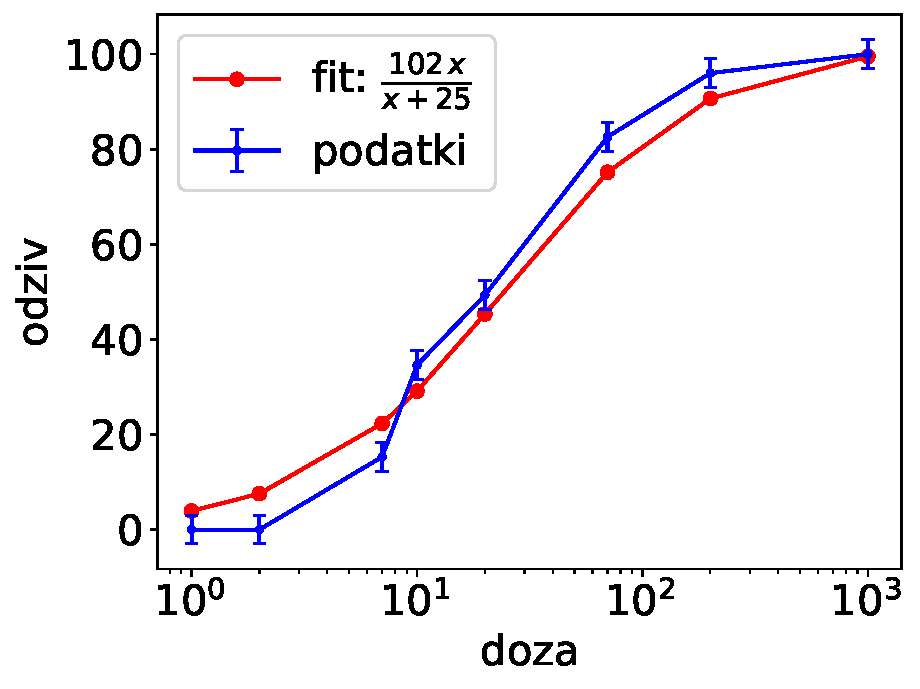
\includegraphics[width=\linewidth]{6. nal slike/rocni_fit_farm.pdf}
        \caption{Ročno ugotovljeni parametri $c_0$ in $\lambda$}
    \end{subfigure}
    \begin{subfigure}{0.5\textwidth}
        \centering
        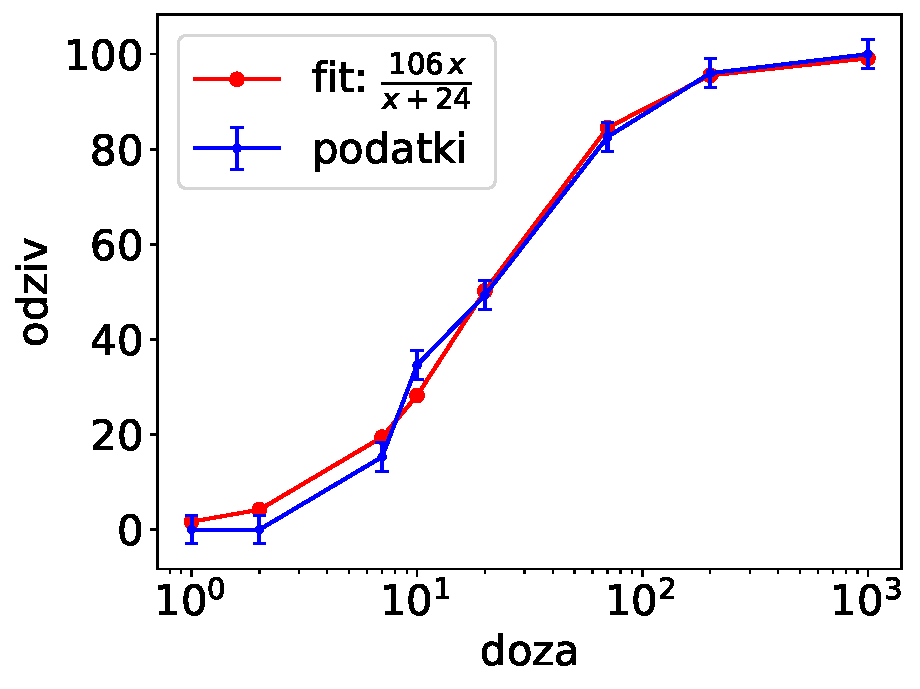
\includegraphics[width=\linewidth]{6. nal slike/LM_farm.pdf}
        \caption{Z metodo Levenberg-Marquardt}
    \end{subfigure}
\end{centering}
\caption{Rešitve za osnoven problem}
\end{figure}

Sistem lahko lineariziramo:
\begin{equation}
    f(x) = \frac{1}{y} = \frac{1}{y_0} + \frac{a}{y_0} \, \frac{1}{x} = \sum_{j=1}^M a_j \, \Phi_j(x)
    \longrightarrow a_1 = \frac{1}{y_0},\, a_2 = \frac{a}{y_0},\, \Phi_1(x) = 1,\, \Phi_2(x)  = \frac{1}{x}
\end{equation}
Pri tem se transformira tudi napaka:
\begin{equation}
    \frac{1}{y \pm \sigma} \approx f(x) \pm \frac{\sigma}{y^2} \longrightarrow \Tilde{\sigma} = \frac{\sigma}{y^2}
\end{equation}
Lineariziran sistem lahko rešimo preprosti z rešitvijo matrične enačbe $A \, \vec{a} = \vec{b}$, kjer je za naš primer število parametrov in dimenzije matrike ter vektorjev enako $M=2$:

\begin{align}
    A_{11} &= \sum_{i=1}^N \frac{1}{\Tilde{\sigma_i}^2}  & b_1 &= \sum_{i=1}^N  \frac{f(x_i)}{\Tilde{\sigma_i}^2} \\ \nonumber
    A_{12} = A_{21} &= \sum_{i=1}^N \frac{1}{x_i \, \Tilde{\sigma_i}^2} & b_2 &= \sum_{i=1}^N  \frac{f(x_i)}{x_i \, \Tilde{\sigma_i}^2} \\ \nonumber
    A_{22} &= \sum_{i=1}^N  \frac{1}{x_i^2 \, \Tilde{\sigma_i}^2} \\ \nonumber
\end{align}
Taka rešitev je predstavljena na spodnji sliki, kjer je za primerjavo pretvorjena nazaj v osnovni (nelinearen) problem. Opazimo, da z linearizacijo celo malo zmanjšamo napako ($\chi^2$), medtem ko jo dodaten parameter $p$ očitno zmanjša še za polovico. Ker znaša tak $\chi_r^2 = 0,34$ je to že zelo nizka vrednost in obstaja verjetnost, da smo precenjevali napake.
\begin{figure}[ht!]
\centering
\begin{minipage}{0.49\textwidth}
    \centering
    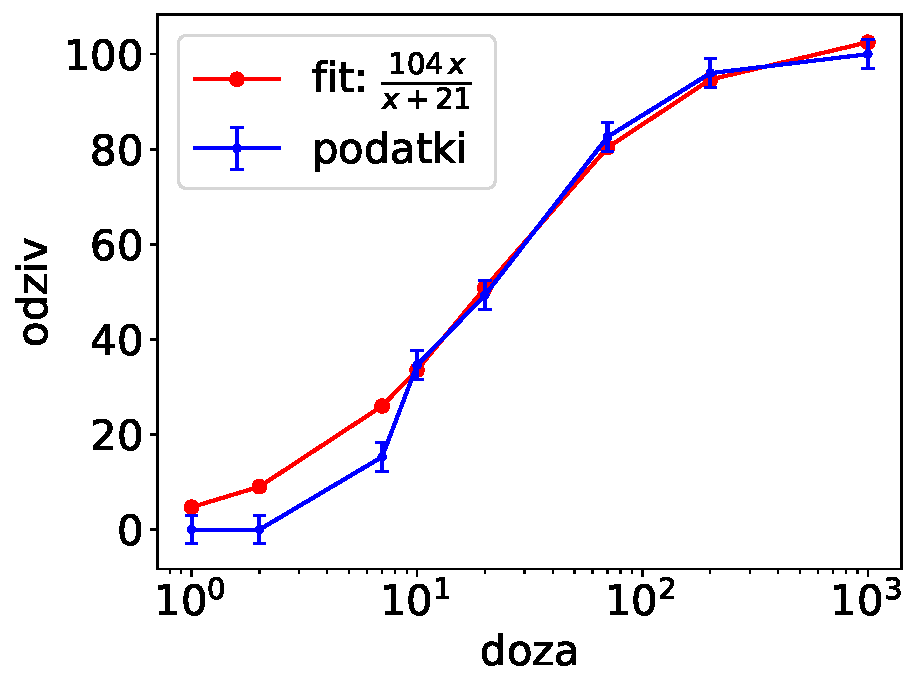
\includegraphics[width=\linewidth]{6. nal slike/matricna_en_farm.pdf}
    \caption{Rešitev za lineariziran problem}
\end{minipage}
\begin{minipage}{0.49\textwidth}
    \centering
    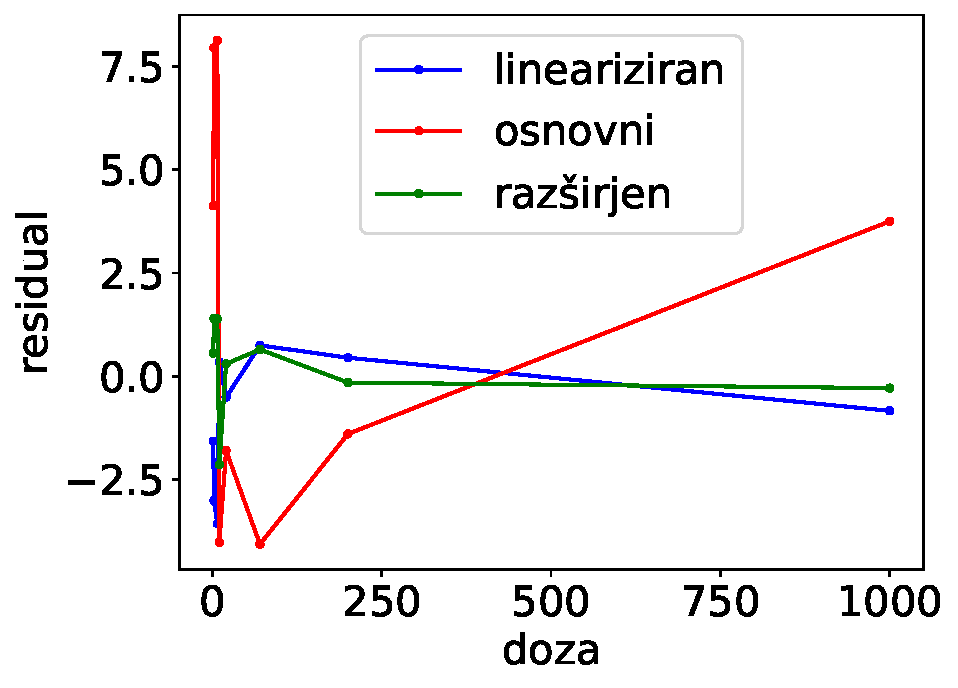
\includegraphics[width=\linewidth]{6. nal slike/napaka_modeli.pdf}
    \caption{Residuali modelov}
\end{minipage}
\end{figure}
\begin{figure}[ht]
    \centering
    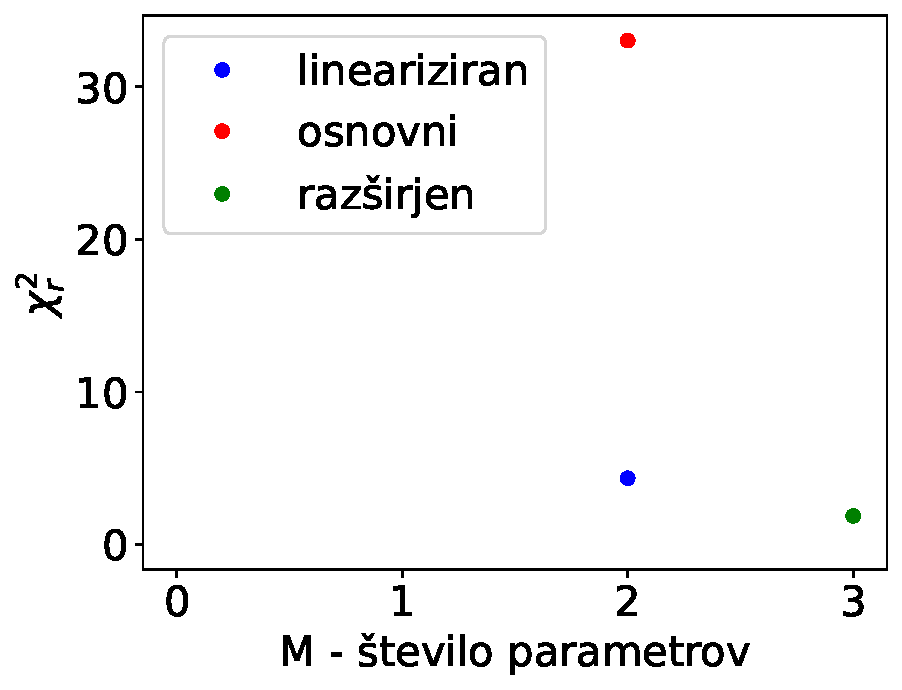
\includegraphics[width=0.5\linewidth]{6. nal slike/chi_farma.pdf}
    \caption{Reduciran $\chi_r^2$}
\end{figure}

\section{Čistilnost ledvic}

Čistilnost ledvic lahko v osnovi opišemo z enorazdelčnim in dvorazdelčnim modelom in jih primerjamo z izmerjenimi podatki. Poskusimo uporabiti tudi več-razdelčne modele.
\begin{align}
    c(t) &= A \, e^{-\lambda \, t} \\ \nonumber
    c(t) &= A \, e^{-\lambda_1 \, t} + B \, e^{-\lambda_2 \, t} \\ \nonumber
    c(t) &= A \, e^{-\lambda_1 \, t} + B \, e^{-\lambda_2 \, t} + C \, e^{-\lambda_3 \, t} \\ \nonumber
    c(t) &= A \, e^{-\lambda_1 \, t} + B \, e^{-\lambda_2 \, t} + C \, e^{-\lambda_3 \, t} + D \, e^{-\lambda_4 \, t} \\ \nonumber
    c(t) &= A \, e^{-\lambda_1 \, t} + B \, e^{-\lambda_2 \, t} + C \, e^{-\lambda_3 \, t} + D \, e^{-\lambda_4 \, t} + E \, e^{-\lambda_5 \, t} \\ \nonumber
\end{align}
Lahko uporabimo tudi konstanto $A_0$, ki popisuje sevanje iz ozadja:
\begin{equation}
    c(t) = A \, e^{-\lambda \, t} + A_0
\end{equation}
in poljubno osnovo eksponenta:
\begin{equation}
    c(t) = A \, osnova^{-\lambda \, t} +A_0
\end{equation}

Ugotovimo, da je za uspešno rešitev potreben ustrezen začetni približek, edinole pri enorazdelčnem modelu z dvema parametroma je še mogoče rešitev dobiti ročno. Ta rešitev predstavlja premico na log y-osi. Z večanjem razdelkov sicer zmanjšujemo napako le do trorazdelčnega modela -- več ni smiselno uporabljati. Ker ne poznamo negotovosti meritev, ne moremo izvesti testa $\chi^2$, lahko pa to naredimo brez deljenja s $\sigma$ in primerjamo le razlike med izračunanimi in izmerjenim vrednostimi ($|y_i - f(x_i)|$), kar smo tudi storili. Skupna napaka modela, dobljena kot absolutna vsota napak izračuna glede na meritev - residualov, ki jih vrne algoritem, z ozadjem sevanja se nahaja med dvo in eno-razdelčno. Zanimivo je, da se z isto napako nahaja tudi model s poljubno osnovo, ki je konvergirala zelo blizu Eulerjevega števila, uporabljenega v drugih modelih. Tako lahko ugotovimo, da upoštevanje sevanja z ozadjem bolje popiše naše izmerke.

\begin{figure}[ht!]
\begin{centering}
    \begin{subfigure}{0.5\textwidth}
        \centering
        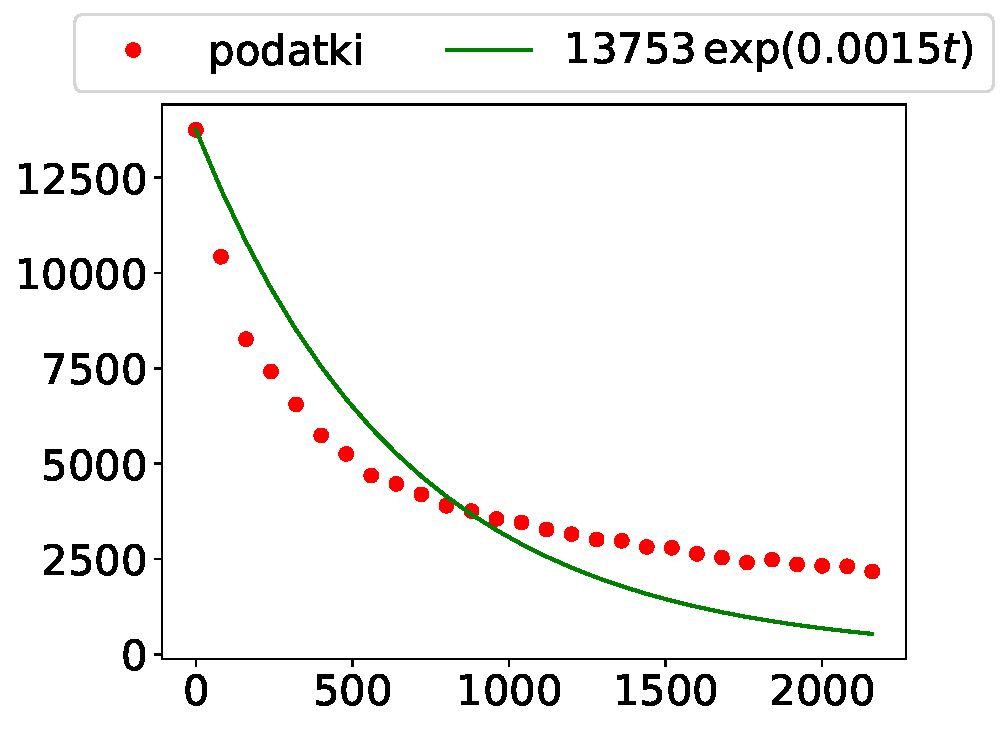
\includegraphics[width=\linewidth]{6. nal slike/ledvice_ročno.pdf}
        \caption{Ročno ugotovljeni parametri}
    \end{subfigure}
    \begin{subfigure}{0.5\textwidth}
        \centering
        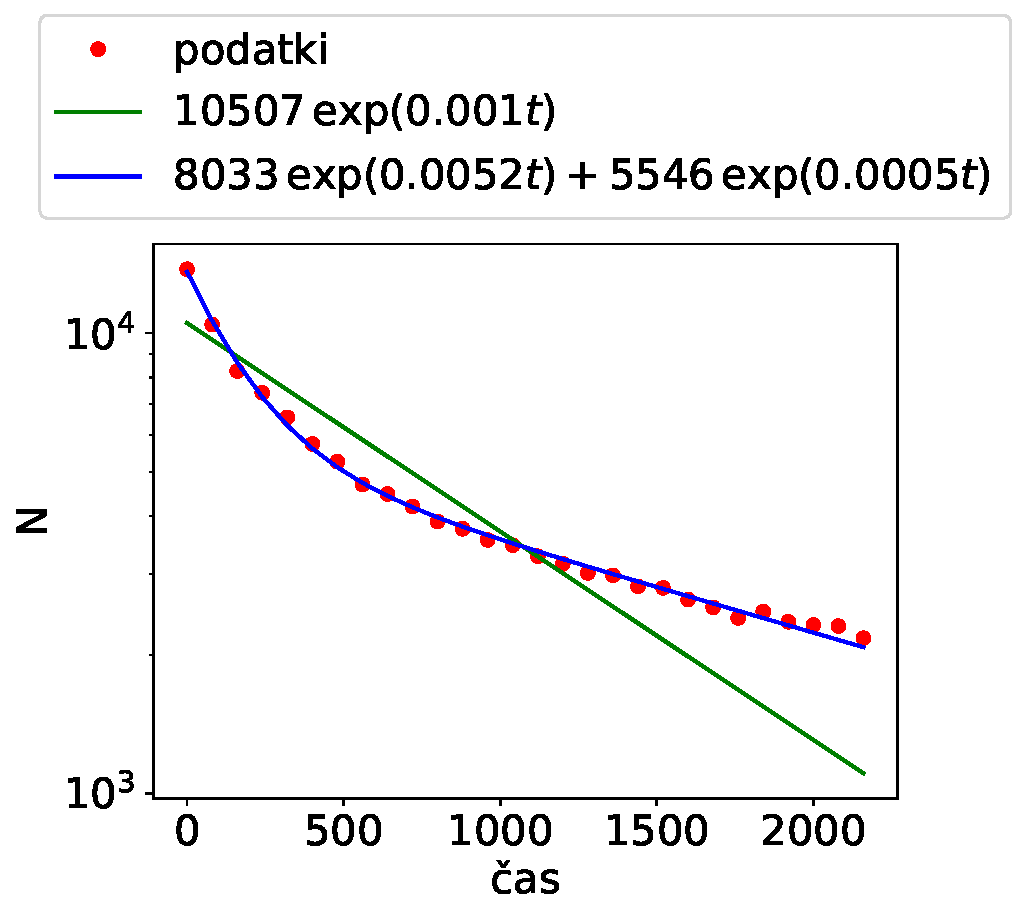
\includegraphics[width=\linewidth]{6. nal slike/ledvice_LM.pdf}
        \caption{Rešitev enorazdelčnega modela z začetnim približkom $C_0 = N[1] = 13753$ in $\lambda = 0,001$ ter dovrazdelčnega z $C_1 = C_2= 1$, $\lambda_1 = 0,01$ in $\lambda_2=0,1$ z metodo Levenberg-Marquardt}
    \end{subfigure}
\end{centering}
    \caption{rešitve enorazdelčnega in dvorazdelčnega modela za čiščenje krvi ledvicah}
\end{figure}

Poleg ozadja smo dodali tudi dva modela s korenskim časom:
\begin{align}
    c(t) &= A \, e^{-\lambda \, \sqrt{t}} \\ \nonumber
    c(t) &= A \, e^{-\lambda_1 \, \sqrt{t}} + B \, e^{-\lambda_2 \, \sqrt{t}}
\end{align}
kjer ima enorazdelčni korenski model občutno manjšo absolutno vsoto napak od navadnega enorazdelčnega. Dvorazdelčni korenski model ne prispeva bistveno k natančnejši rešitvi, saj se dogaja enako, kot pri višanju razdelkov navadnih razdelčnih modelov nad tri.
\begin{figure}[ht!]
    \centering
    \begin{minipage}{0.49\textwidth}
        \centering
        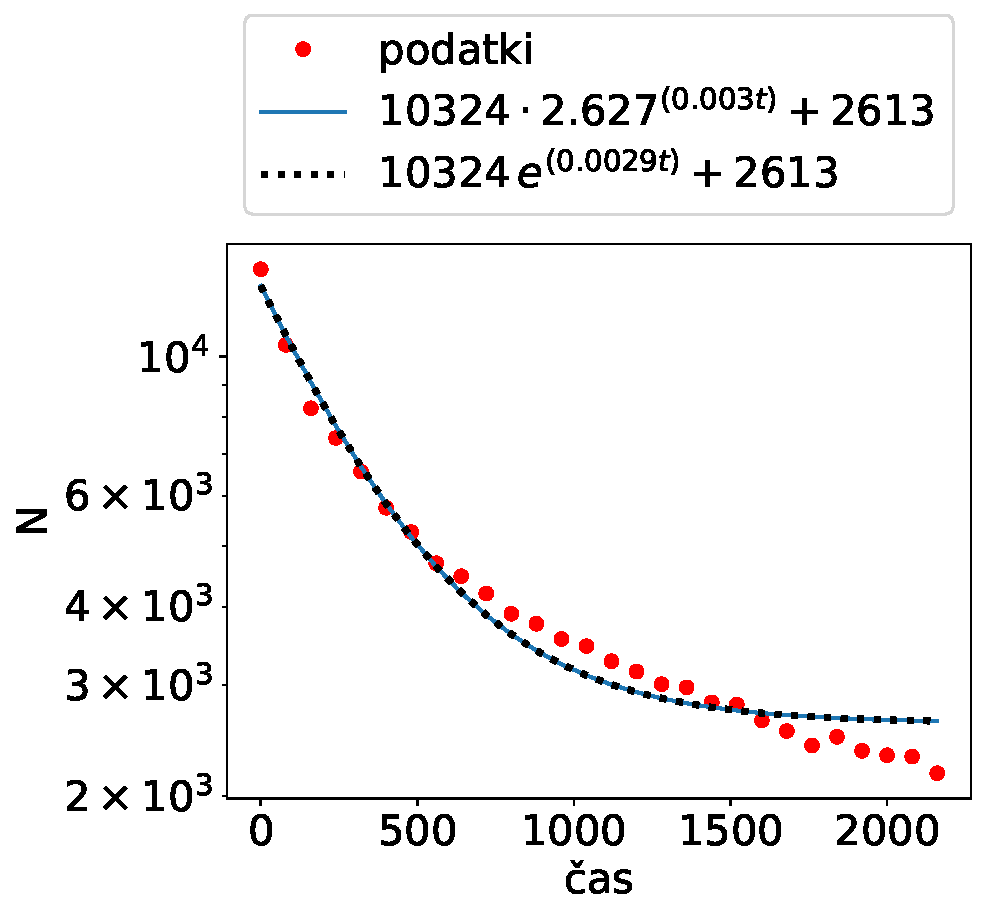
\includegraphics[width=\linewidth]{6. nal slike/ledvice_osnova.pdf}
        \caption{Uporaba poljubne osnove pri sevanju iz ozadja.}
    \end{minipage}
    \begin{minipage}{0.49\textwidth}
        \centering
        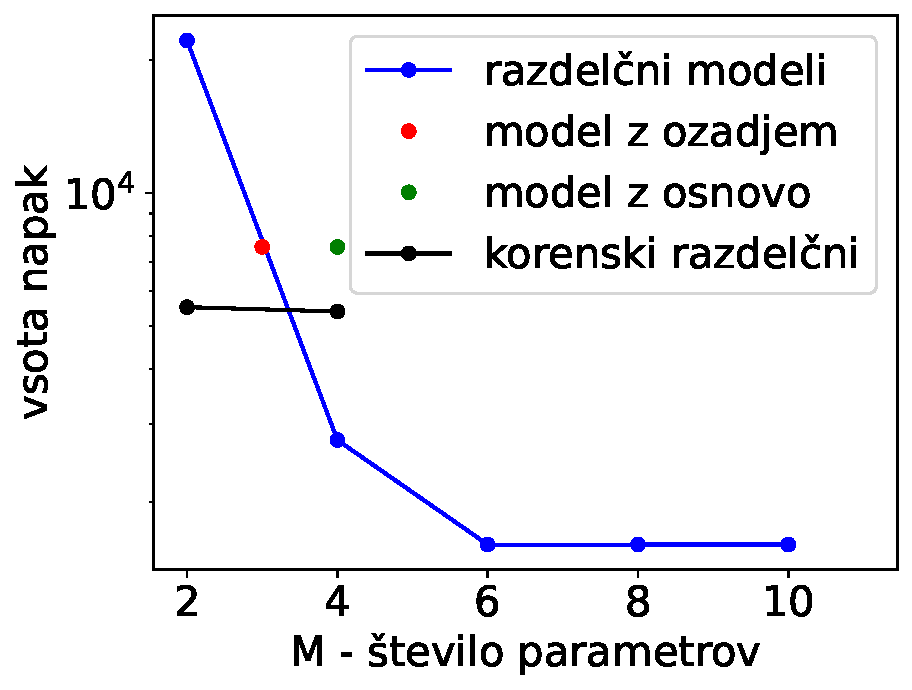
\includegraphics[width=\linewidth]{6. nal slike/ledvica_napaka_param.pdf}
        \caption{Odvisnost absolutne vsote napak od modelov in števila parametrov}
    \end{minipage}
\end{figure}

\begin{figure}[ht!]
    \centering
    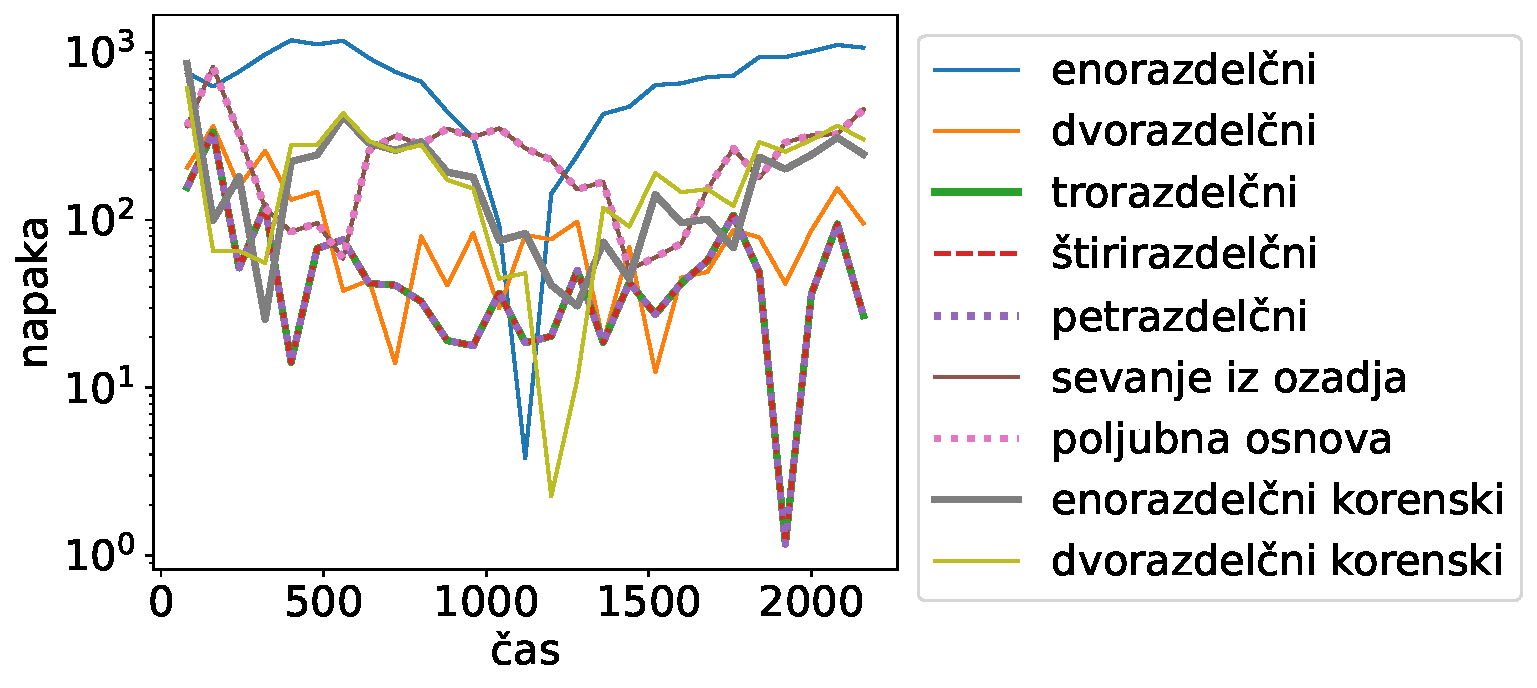
\includegraphics[width=0.75\textwidth]{6. nal slike/ledvice_LM_napake.pdf}
    \caption{Napaka pri uporabi več razdelkov  različnih metod}
\end{figure}

Poskusili smo tudi ``fitati'' polinome na dobljene podatke. Pri tem smo uporabili knjižnico \texttt{NumPy} in rutini \texttt{polyfit} in \texttt{poly1d}. Pri tem opazimo, da višanje reda bolj natančno popiše funkcijo, vendar je z tak popis dovolj točen le na območju definiranih podatkov, saj polinom izven njih le bolj ``pobezlja''. Napaka rešitve se asimptotsko približuje nični, na logaritemski skali pa je začuda viden skok, katerega vzrok nam ni znan.

Opazimo, da polinomi ne popisujejo pravilno fizikalnega dogajanja. Napaka tako dobljene rešitve je pri enakem številu parametrov kot pri razdelčnih modelih lahko za nekaj velikostnih razredov višja, vendar so vseeno uporabni, če ne poznamo boljšega funkcijskega popisa.
\begin{figure}[H]
    \centering
    \begin{minipage}{0.49\textwidth}
        \centering
        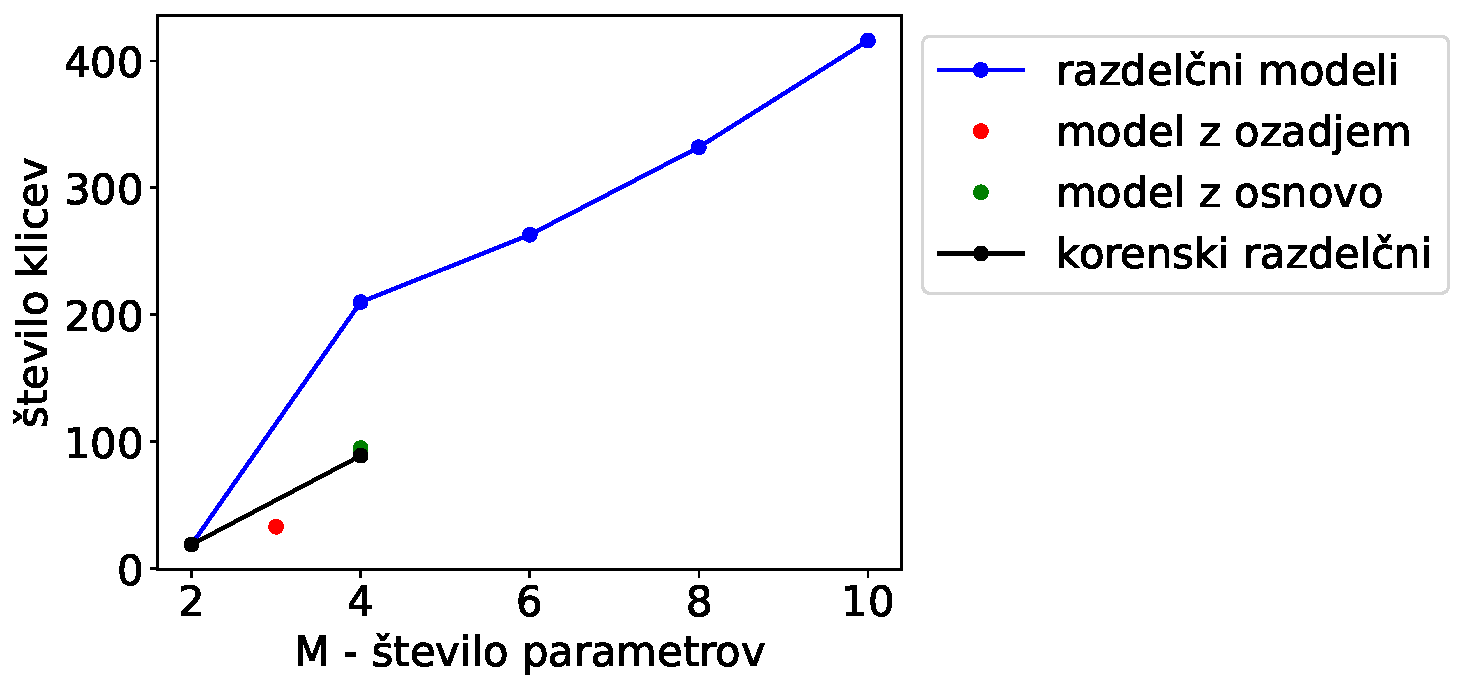
\includegraphics[width=\linewidth]{6. nal slike/ledvice_st_klicev.pdf}
        \caption{Odvisnost števila klicev funkcije znotraj LM algoritma}
    \end{minipage}
    \begin{minipage}{0.49\textwidth}
        \centering
        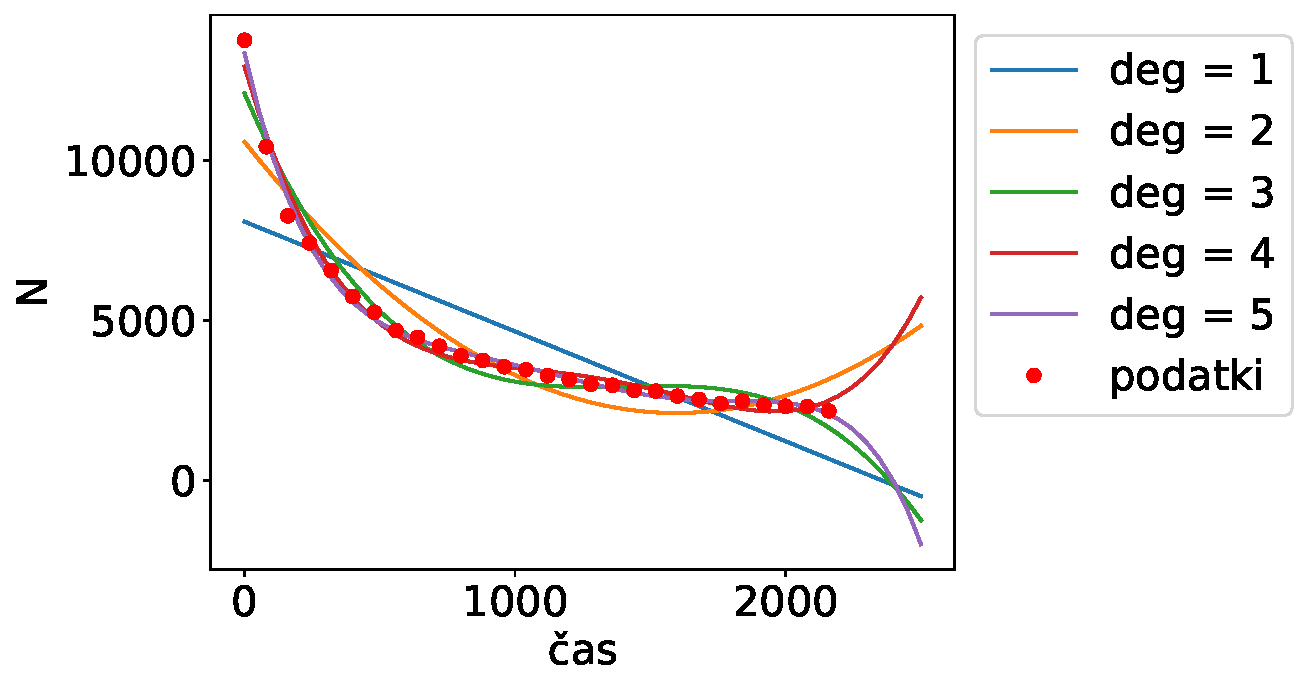
\includegraphics[width=\linewidth]{6. nal slike/ledvice_poli.pdf}
        \caption{Uporaba polinomskih funkcij}
    \end{minipage}
\end{figure}
\begin{figure}[H]
    \centering
    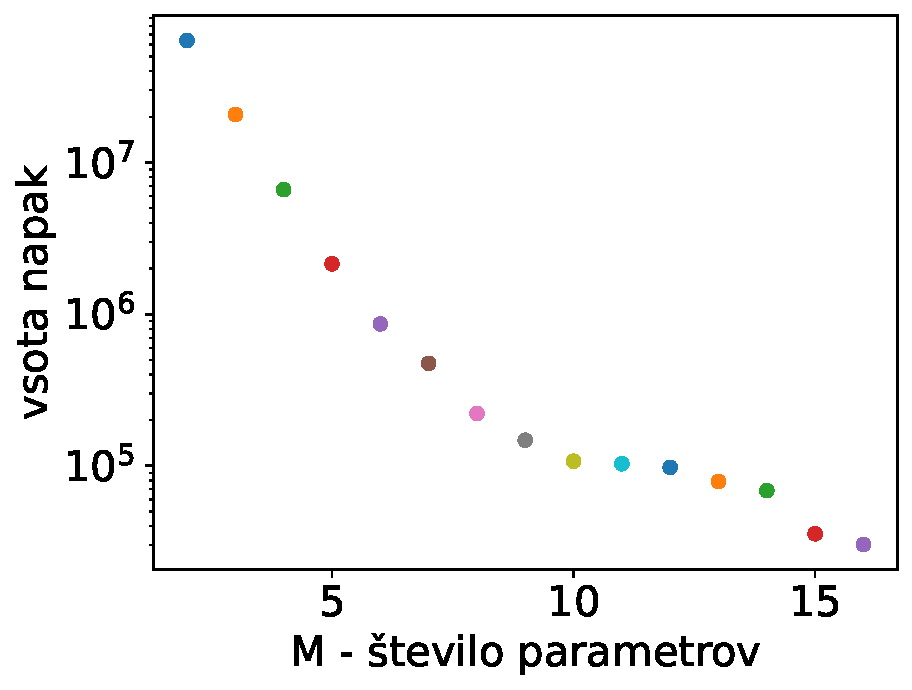
\includegraphics[width=0.37\linewidth]{6. nal slike/ledvice_napaka_poli.pdf}
    \caption{Absolutna vsota napak polinomov do 15. reda}
\end{figure}


\section{Magnetni spektrometer}

Lahko uporabimo spodnjo splošno enačbo za popis odvisnosti začetnega kota $\theta_{tg}$ od kota $\theta_{fp}$ in lege $x_{fp}$ na detektorju:
\begin{equation}
    \theta_{tg}(x_{fp},\theta_{fp}) = \sum_{i=0}^N \, \left[ \sum_{j=0}^M \, a_{i,j} \, x_{fp}^j \right] \, \theta_{fp}^i
\end{equation}
kjer je $M$ red polinoma za popis odvisnosti $\theta_{tg}(x_{fp})$ in $N$ za  $\theta_{tg}(\theta_{fp})$. Tako dobimo najosnovnejšo enačbo takrat, ko oba polinoma razvijemo do prvega reda:
\begin{equation}
    \theta_{tg}(x_{fp},\theta_{fp}) = (a_{00} + a_{01}\,x_{fp}) + (a_{10} + a_{11}\,x_{fp})\,\theta_{fp}
\end{equation}

Za reševanje takega sistema uporabljamo singularni razcep (SVD), ki je v Pythonu implementiran v funkciji \texttt{numpy.linalg.lstsq}. Da preverimo delovanje algoritma, smo izvedli rekonstrukcijo znane sedlaste funkcije $$f(x,y) = a_0 + a_1 \, x^2 + a_3 \, y^2, $$ ki smo ji lahko dodatno dodali naključen šum med (-1, 1), pomnožen s stopnjo zašumljenosti.

Opazili smo, da $\chi^2$ eksponentno narašča z večanjem šuma, drugače pa algoritem lepo prilagodi funkcijo podatkom. V primeru brez šuma dobimo zalo majhno vrednost $\chi_r^2$ reda $10^{-27}$.

\begin{figure}[ht]
\centering
\begin{subfigure}{0.49\textwidth}
    \centering
    \includegraphics[width=\linewidth]{6. nal slike/test_svd_0.pdf}
    \caption{Testna funkcija brez šuma}
\end{subfigure}
\begin{subfigure}{0.49\textwidth}
    \centering
    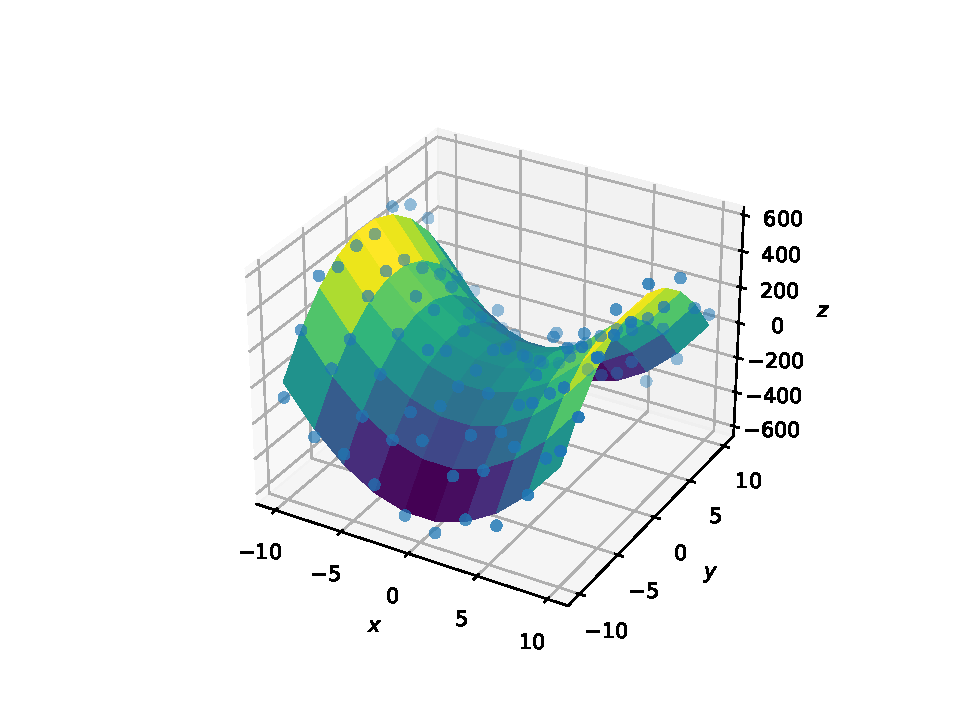
\includegraphics[width=\linewidth]{6. nal slike/test_svd_100šum.pdf}
    \caption{Testna funkcija s šumom}
\end{subfigure}
\end{figure}
\begin{figure}[ht]
    \centering
    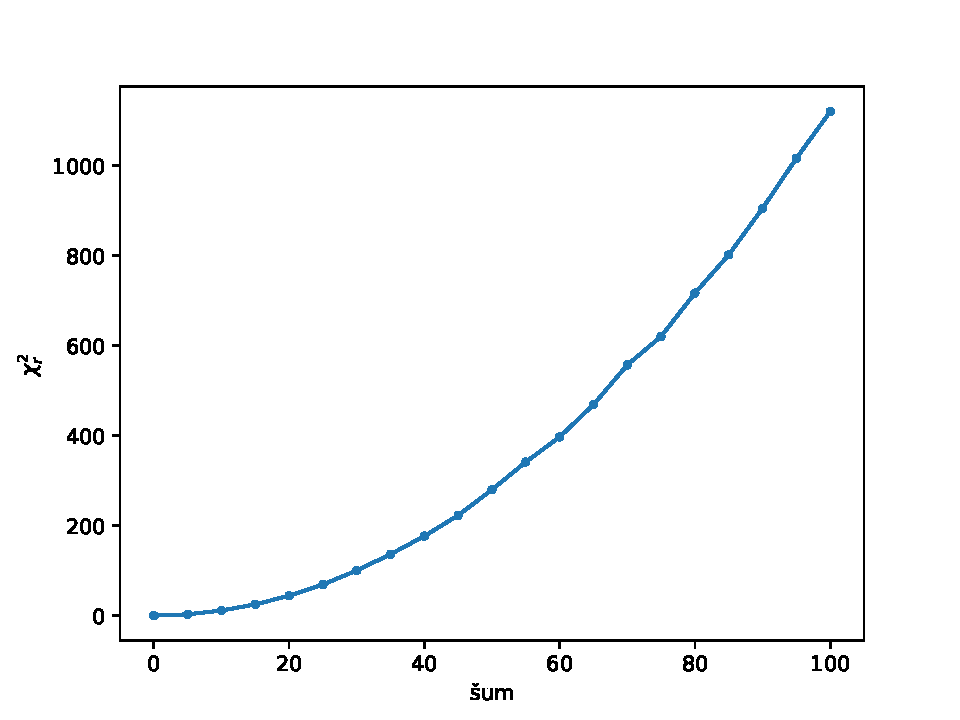
\includegraphics[width=0.75\linewidth]{6. nal slike/test_svd_šum_chi.pdf}
    \caption{Odvisnost reduciranega $\chi_r^2$ od stopnje zašumljenosti}
\end{figure}

Sedaj lahko analiziramo podatke iz datoteke. Ugotovimo, da se presenetljivo višanje redov polinomov za popis ne odraža v bolj točni rešitvi, temveč ravno obratno; polinomi višjih redov PODIVJAJO. 

\begin{figure}[H]
    \centering
    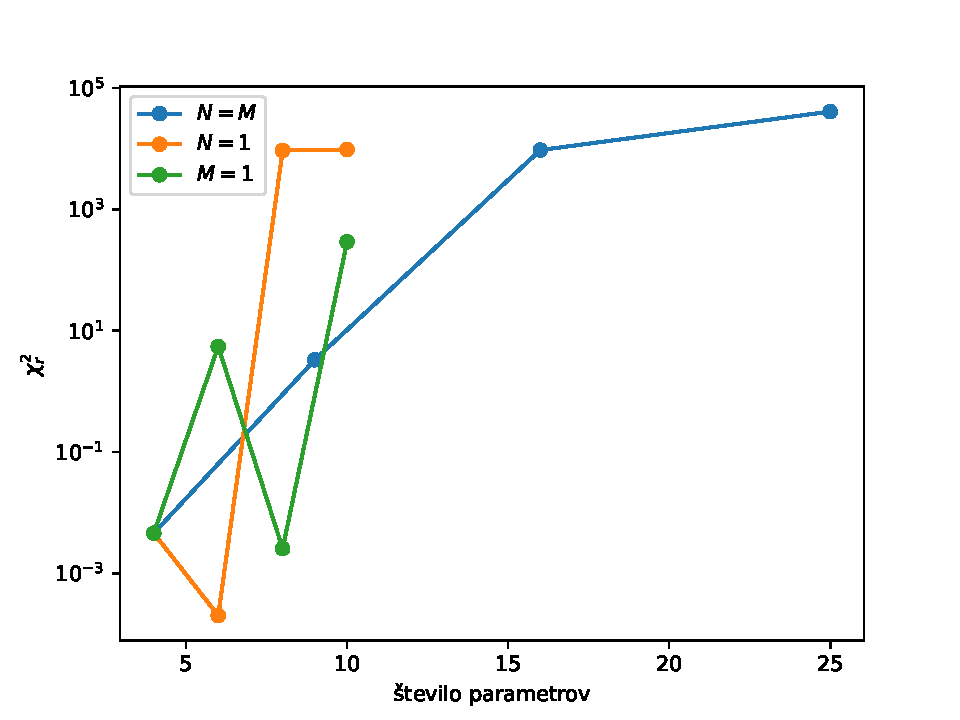
\includegraphics[width=0.7\linewidth]{6. nal slike/spektro_napake_vse.pdf}
    \caption{$\chi_r^2$ za vse primere polinomov do 4. reda za $N$ in $M$}
\end{figure}

\begin{figure}[H]
\centering
\begin{subfigure}{0.49\textwidth}
    \centering
    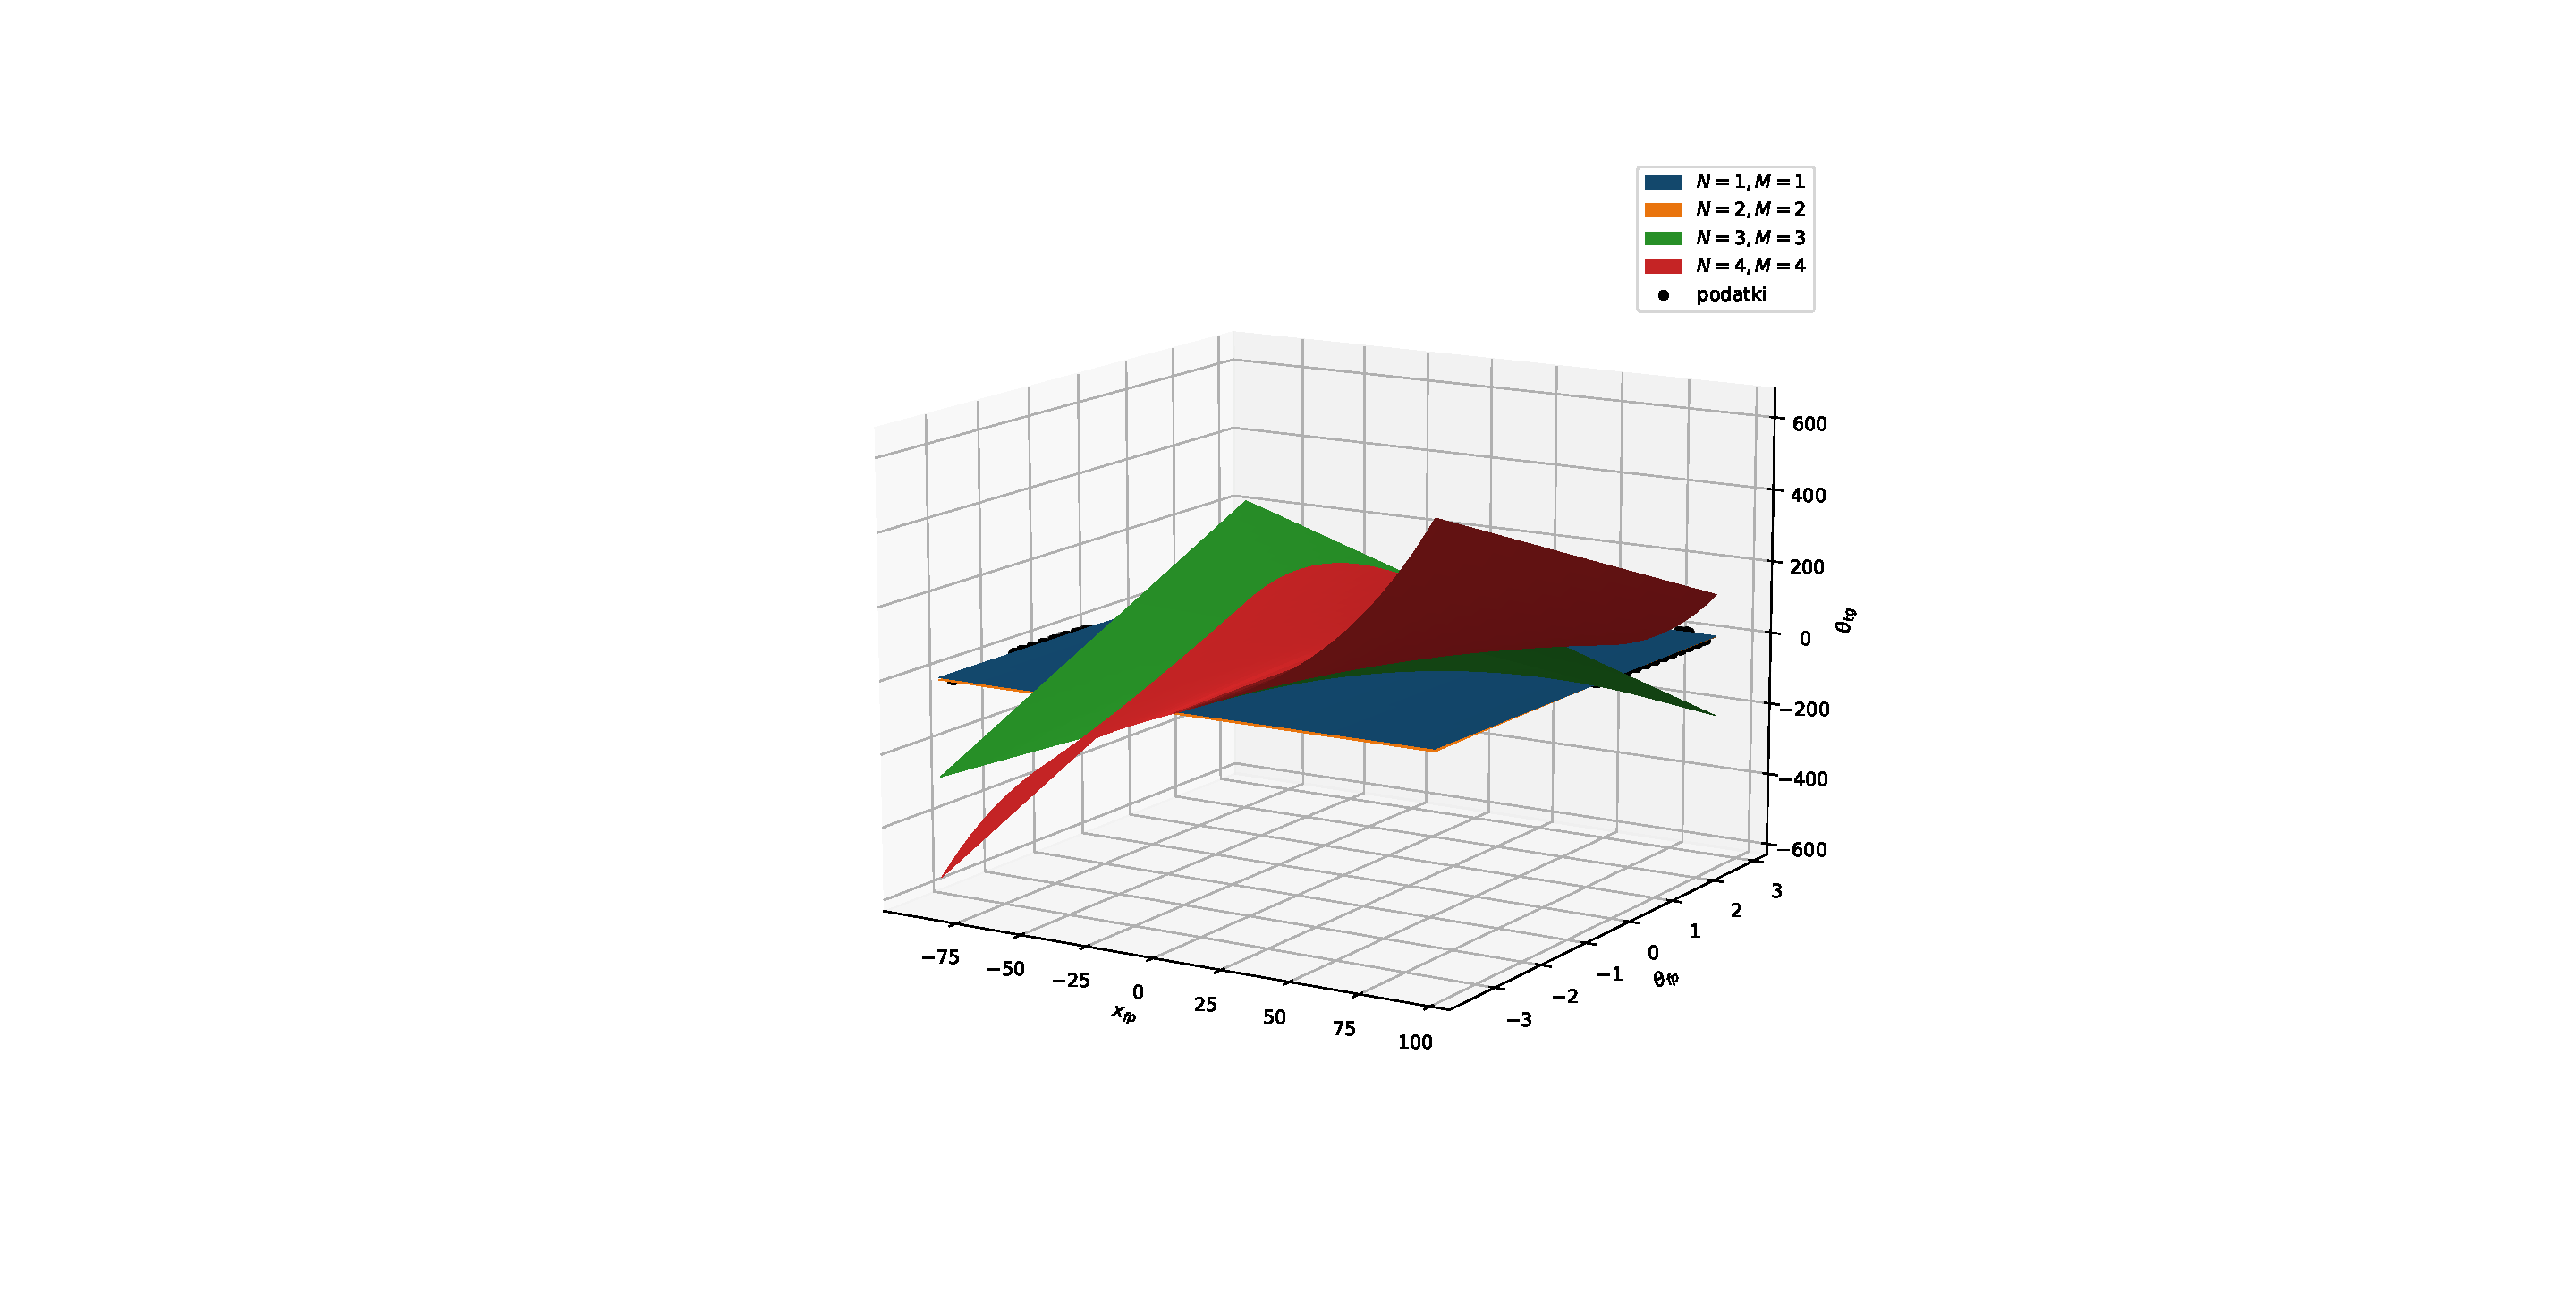
\includegraphics[width=\linewidth]{6. nal slike/spektro_isti_redi.pdf}
\end{subfigure}
\begin{subfigure}{0.49\textwidth}
    \centering
    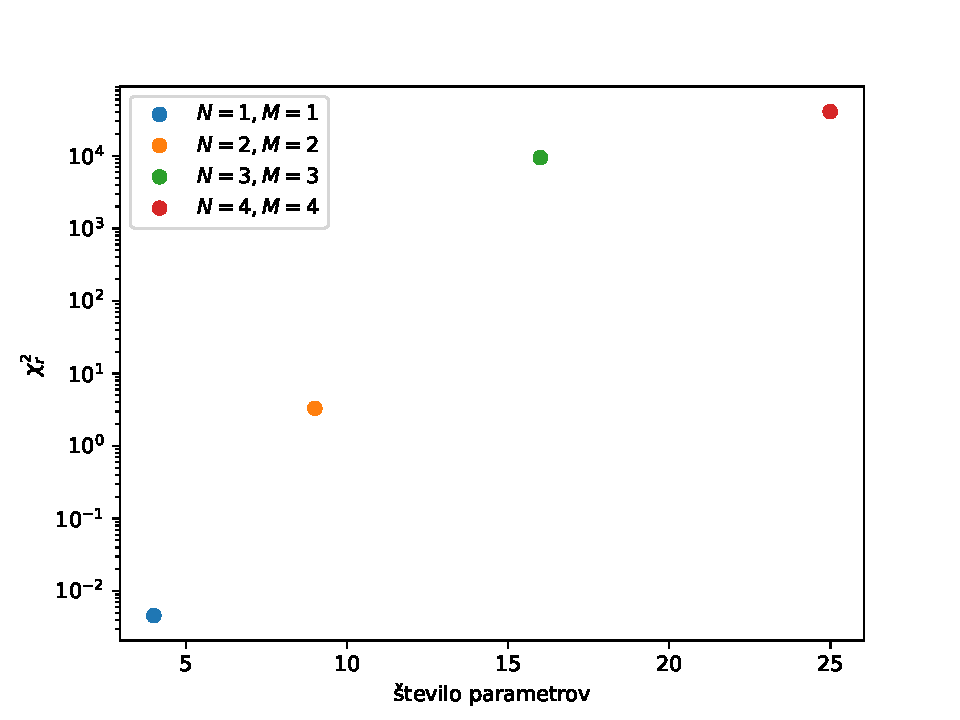
\includegraphics[width=\linewidth]{6. nal slike/spektro_isti_redi_napaka.pdf}
\end{subfigure}
    \caption{Polinomi z enakimi redi $M=N$}
\end{figure}

\begin{figure}[H]
\centering
\begin{subfigure}{0.49\textwidth}
    \centering
    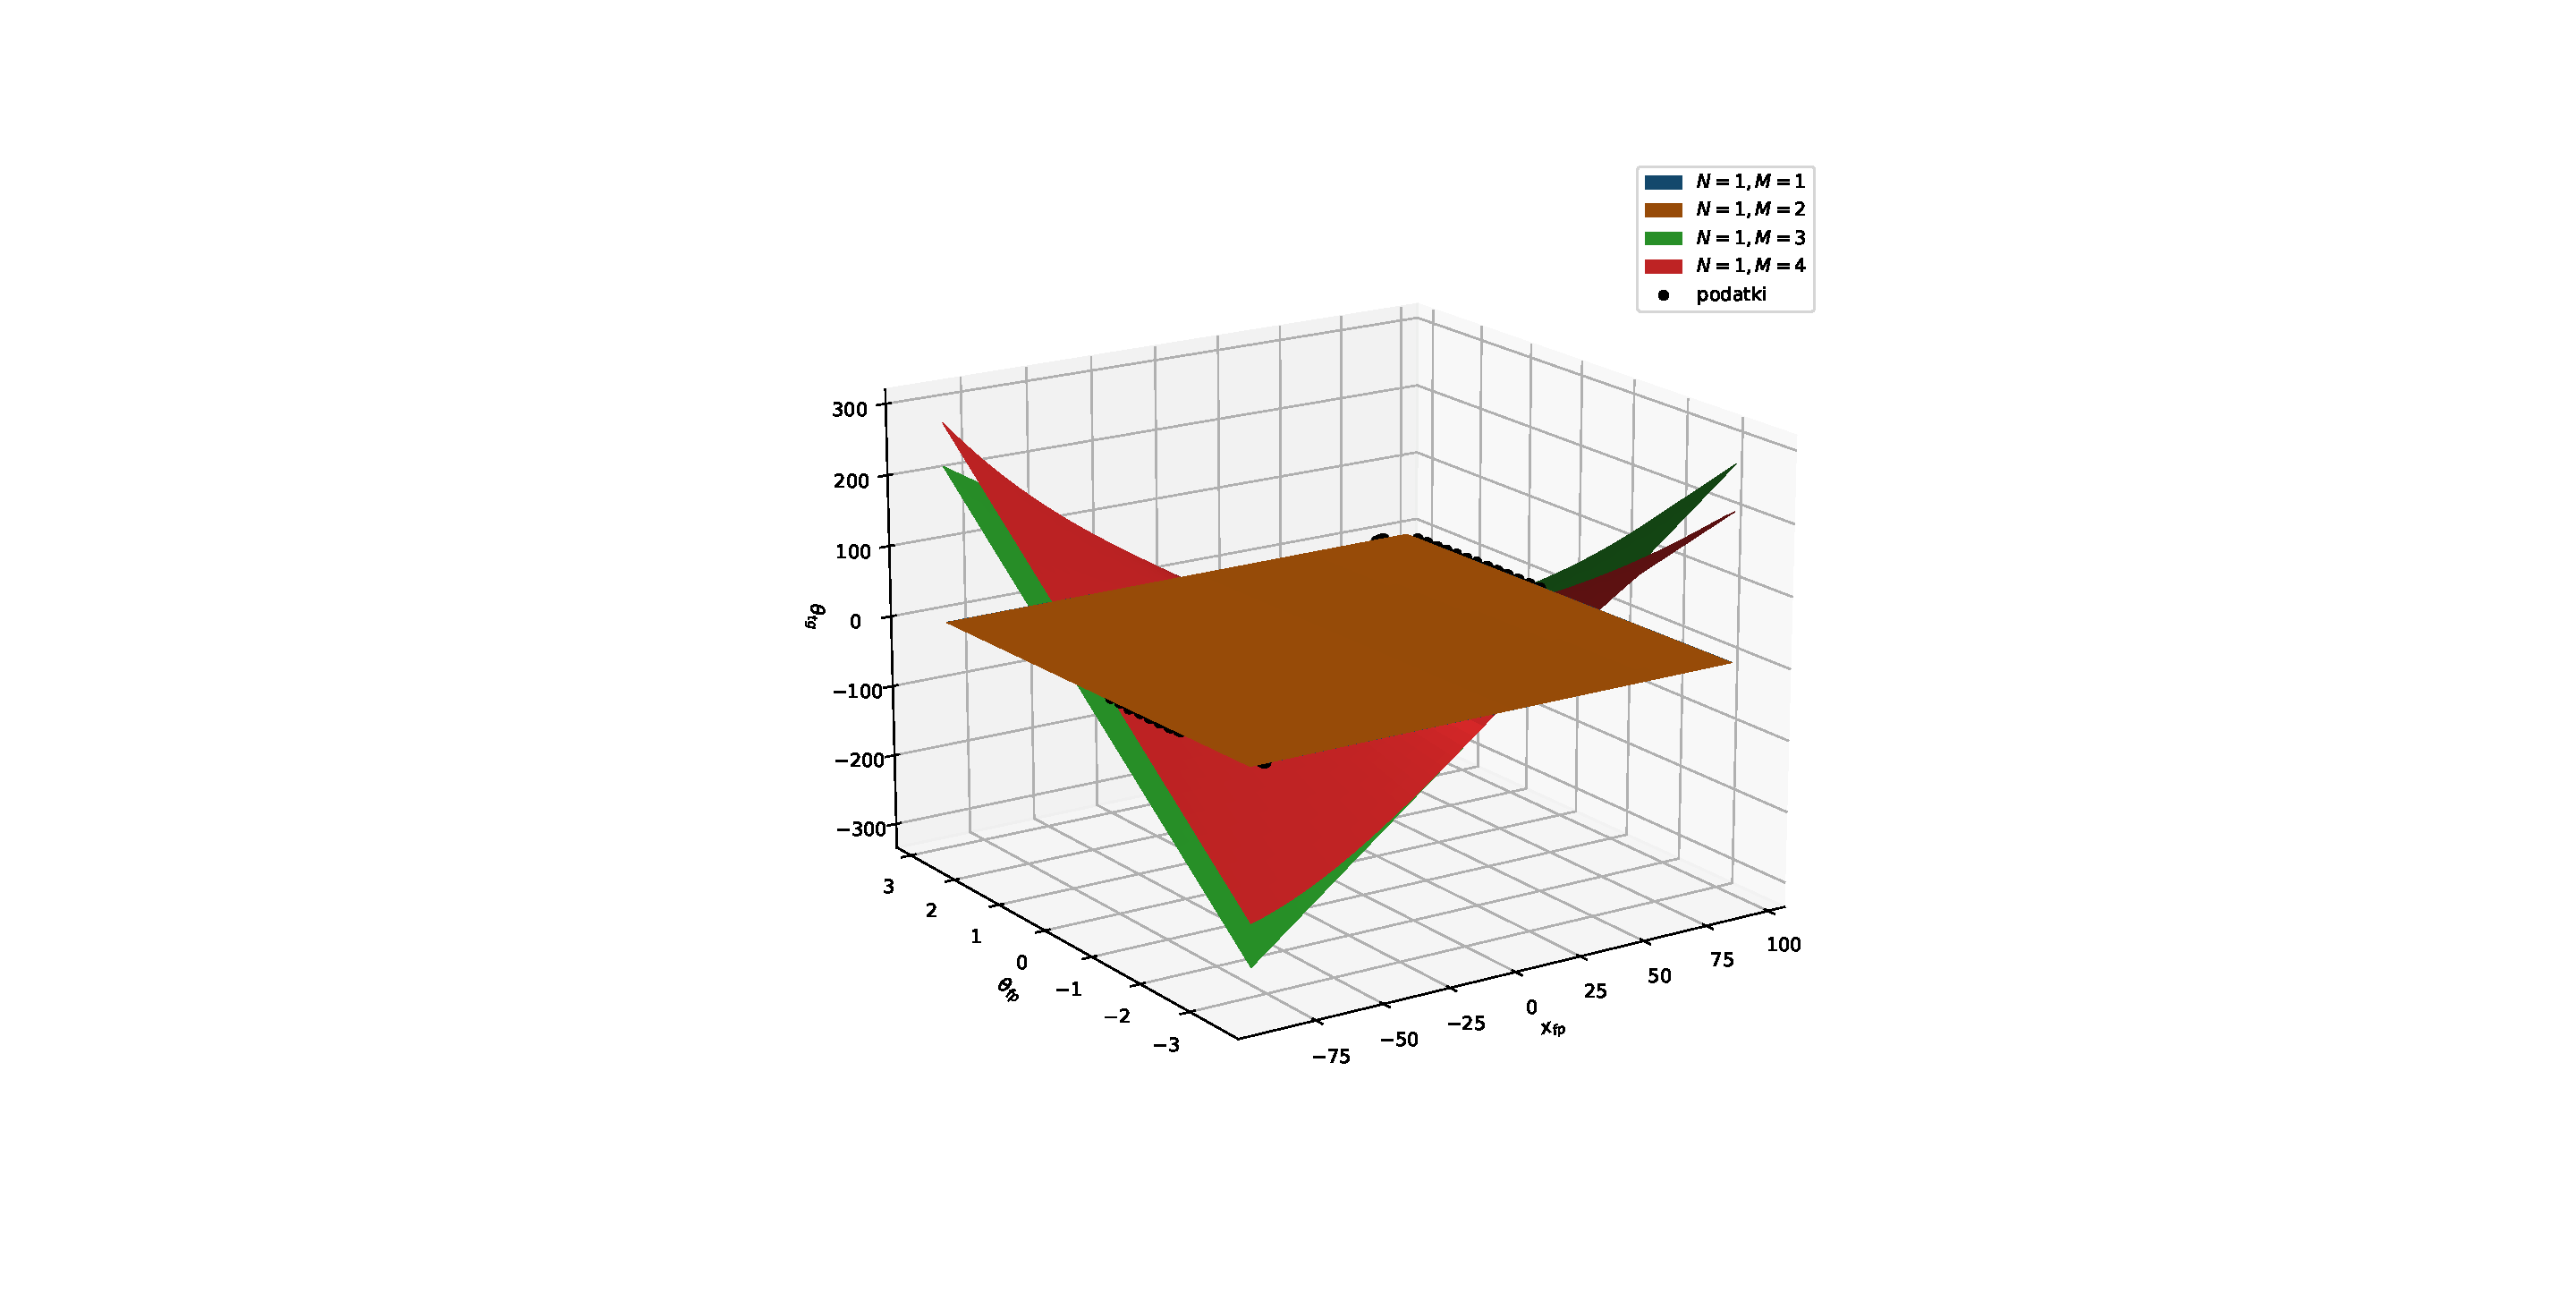
\includegraphics[width=\linewidth]{6. nal slike/spektro_M.pdf}
\end{subfigure}
\begin{subfigure}{0.49\textwidth}
    \centering
    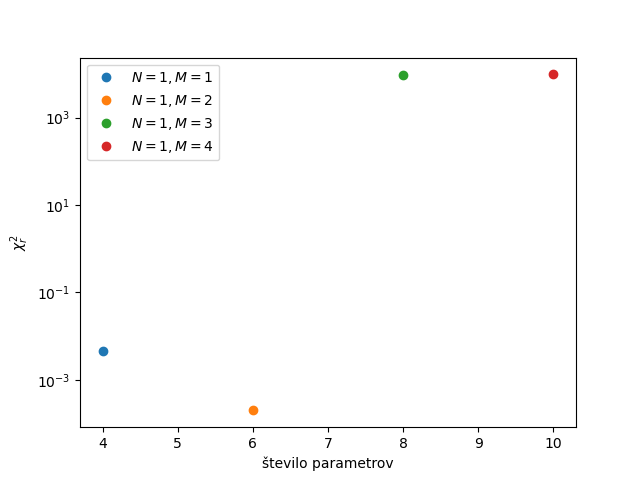
\includegraphics[width=\linewidth]{6. nal slike/spektro_M_napake.png}
\end{subfigure}
    \caption{Polinomi z različnimi redi $M$ pri fiksnem $N=1$}
\end{figure}

\begin{figure}[H]
\centering
\begin{subfigure}{0.49\textwidth}
    \centering
    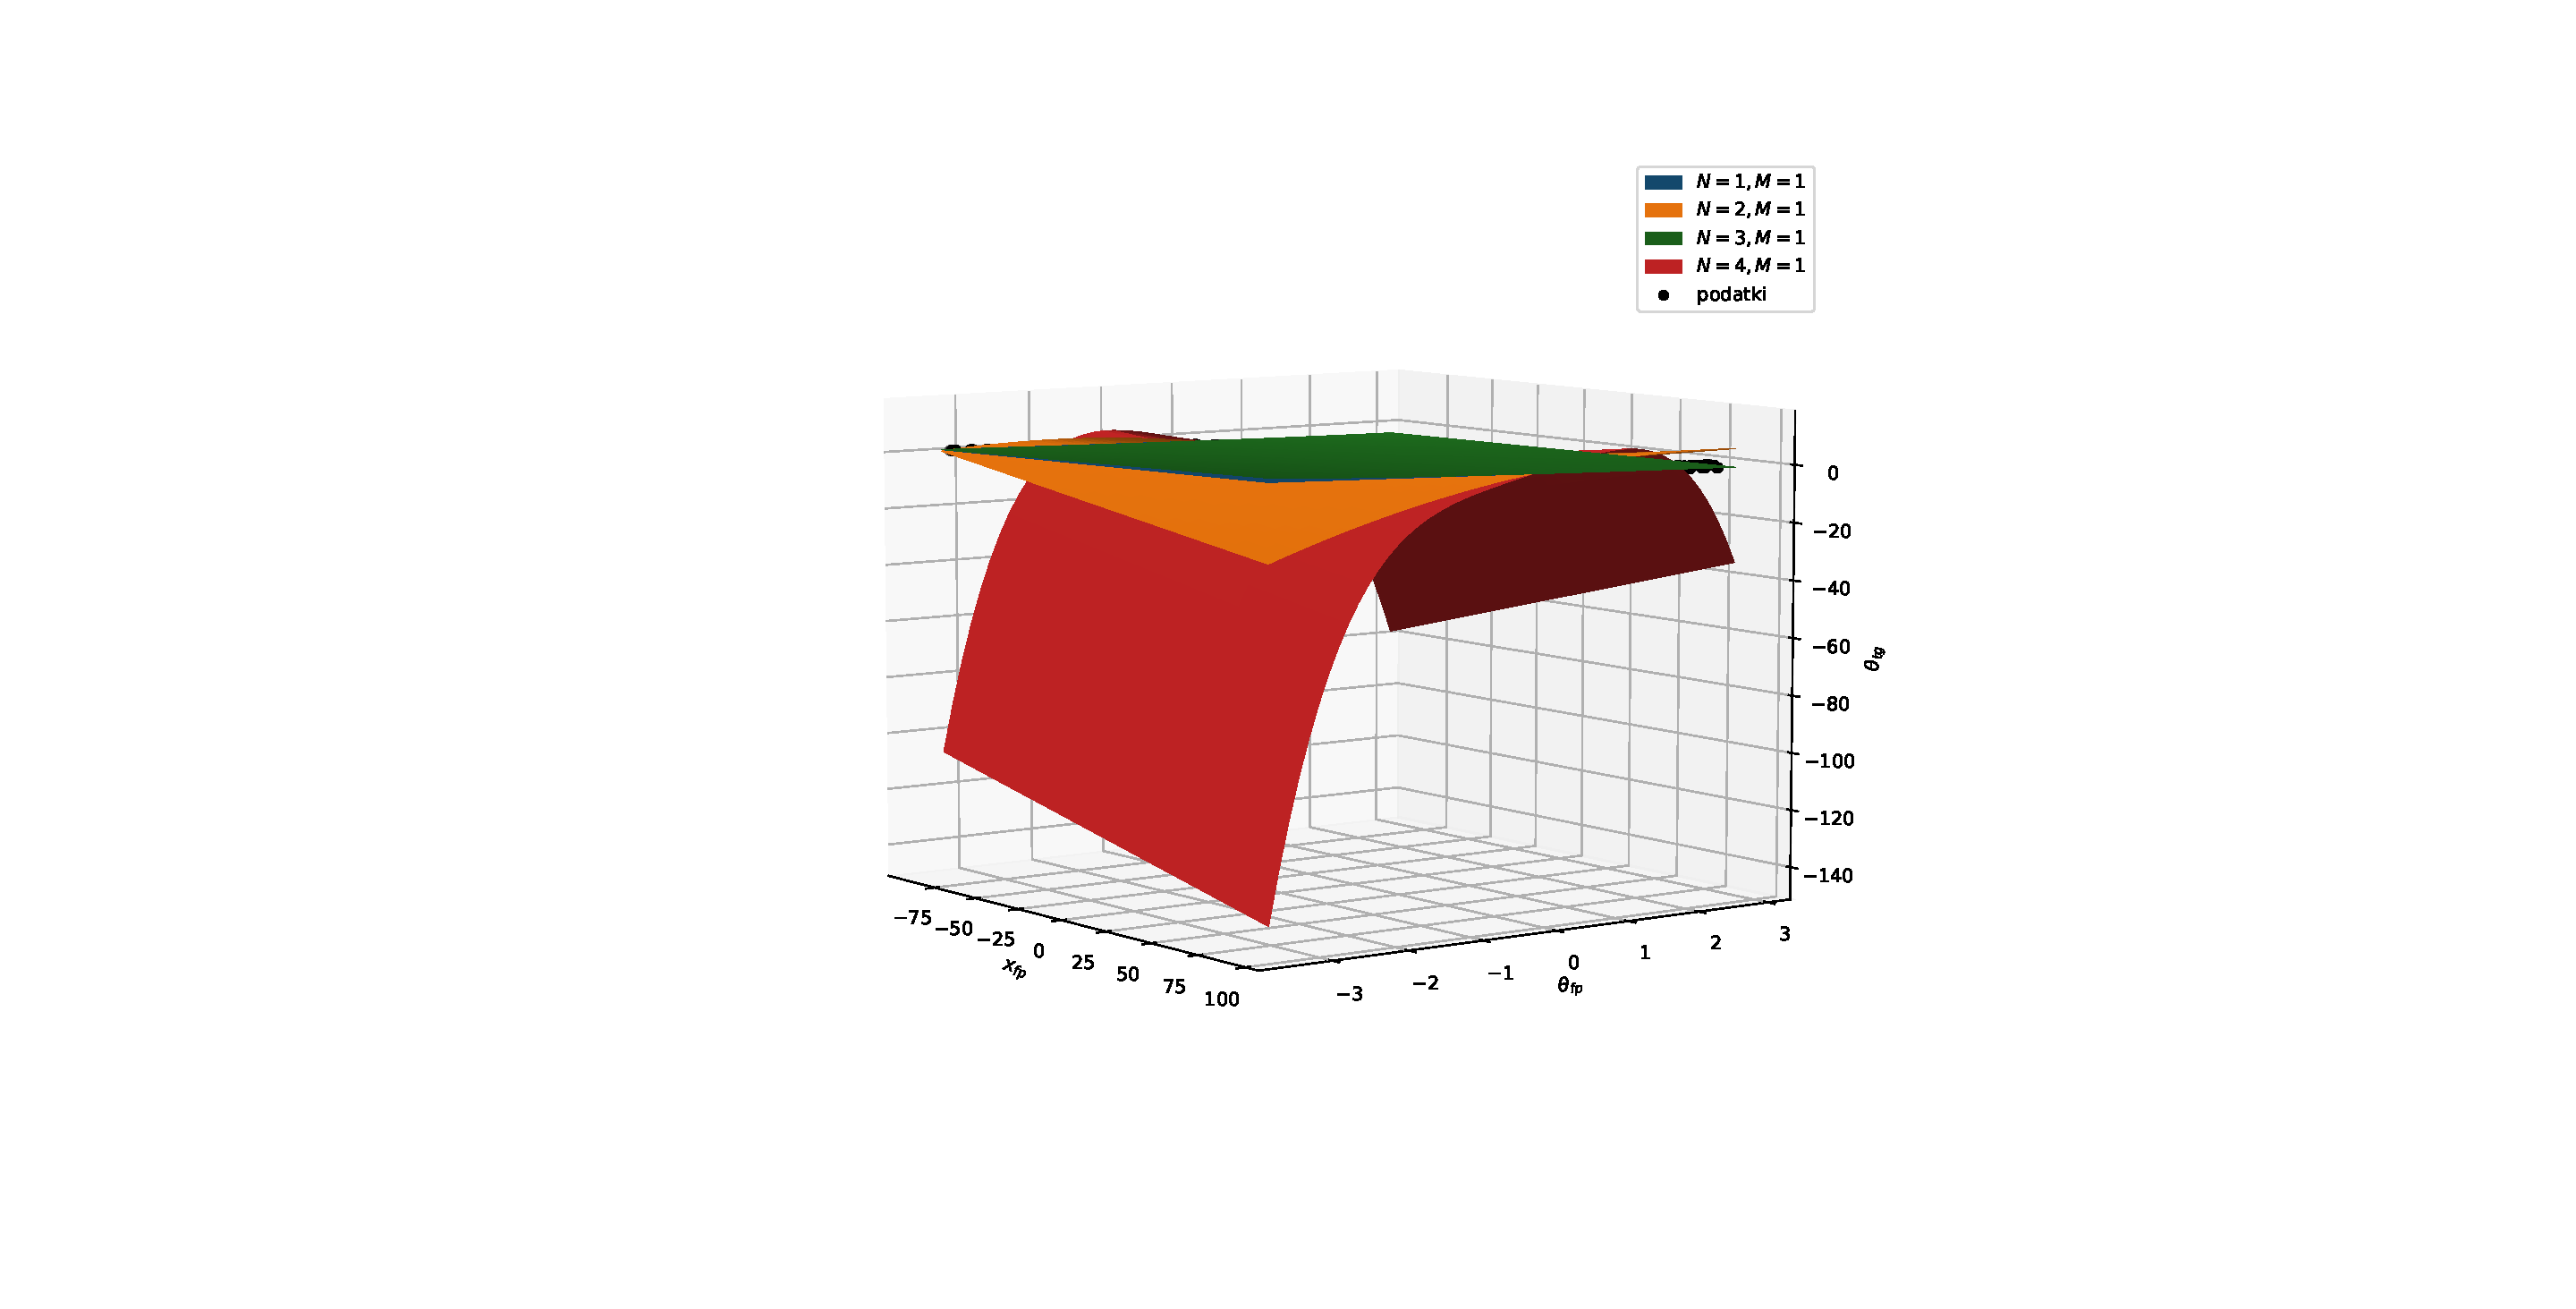
\includegraphics[width=\linewidth]{6. nal slike/spektro_N.pdf}
\end{subfigure}
\begin{subfigure}{0.49\textwidth}
    \centering
    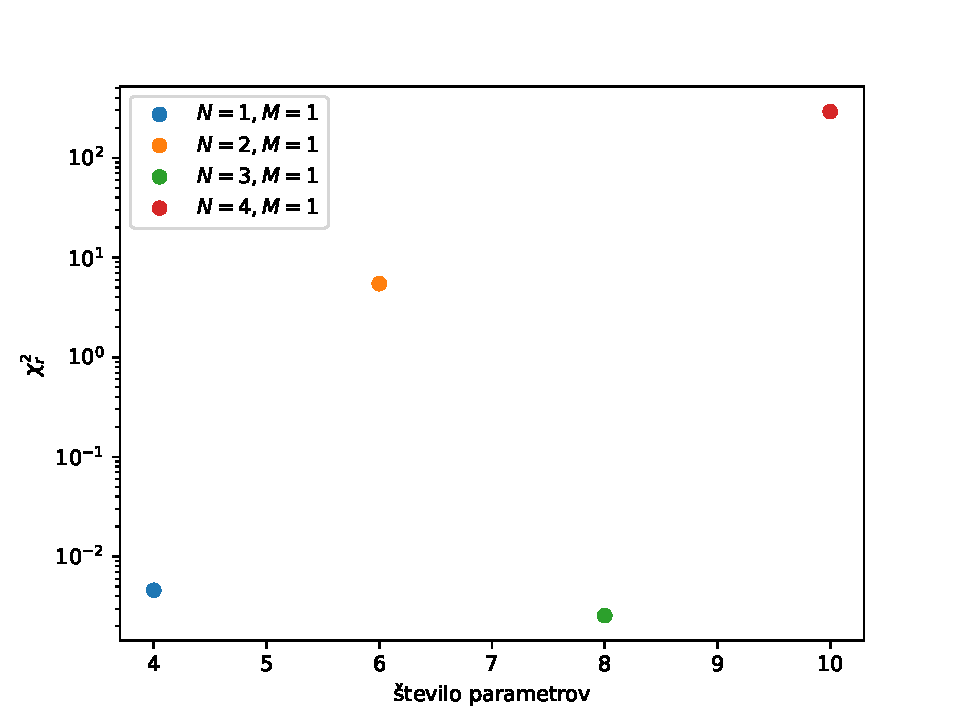
\includegraphics[width=\linewidth]{6. nal slike/spektro_N_napake.pdf}
\end{subfigure}
    \caption{Polinomi z različnimi redi $N$ pri fiksnem $M=1$}
\end{figure}

\newpage
Vidimo, da v primeru ko $N=1$ in $M=2$ dobimo najbolj podatkom prilegajoč se popis, ko je $\chi_r^2 = 2,0\, 10^{-4}$, ki ga opisuje spodnja enačba. Sledi drugi najboljši popis $N=3$ in $M=1$, ko $\chi_r^2 = 2,6\, 10^{-3}$ in tretji (in hkrati najenostavnejši) popis z ravnino $N=M=1$, kjer je $\chi_r^2 = 4,6\, 10^{-3}$.

\begin{equation}
    \theta_{tg}(x_{fp},\theta_{fp}) = (a_{00} + a_{01}\,x_{fp} + a_{02}\,x_{fp}^2) + (a_{10} + a_{11}\,x_{fp} + a_{12}\,x_{fp}^2)\,\theta_{fp}
\end{equation}

\begin{table}[ht]
    \centering
    \begin{tabular}{c|c|c}
        a & vrednost & singularna vrednost \\
        \hline
        $a_{00}$ & ~1,66$\,10^{-2}$ & 982 830 \\
        $a_{01}$ & ~1,71$\,10^{-2}$ & 542 352 \\
        $a_{02}$ & -3,19$\,10^{-5}$ & ~~~5 945 \\
        $a_{10}$ & -0,854~~~~~ & ~~~3 624 \\
        $a_{11}$ & -8,63$\,10^{-6}$ & ~~~~~~~66 \\
        $a_{12}$ & ~1,25$\,10^{-6}$ & ~~~~~~~61 \\
    \end{tabular}
    \caption{Vrednost in pomembnost parametrov izbranega modela}
\end{table}

Iz zgornjih podatkov lahko sklepamo, da so najmanj pomembni zadnji parametri, zato jih lahko postopoma odstranjujemo in spremljamo model. Iz tega dobimo model, okleščen za zadnja dva parametra, torej je odvisnost od $\theta_{fp}$ linearna.

\begin{table}[ht]
    \centering
    \begin{tabular}{c|c|c}
        enačba modela & $\chi_r^2$ & relativna napaka \\
        \hline
        $(a_{00} + a_{01}\,x_{fp} + a_{02}\,x_{fp}^2) + (a_{10} + a_{11}\,x_{fp} + a_{12}\,x_{fp}^2)\,\theta_{fp}$ & 2,0086$\,10^{-4}$ & 0 \% \\
        $(a_{00} + a_{01}\,x_{fp} + a_{02}\,x_{fp}^2) + (a_{10} + a_{11}\,x_{fp})\,\theta_{fp}$ & 2,1748$\,10^{-4}$ & 8,27 \% \\
        $(a_{00} + a_{01}\,x_{fp} + a_{02}\,x_{fp}^2) + a_{10}\,\theta_{fp}$ & 2,1793$\,10^{-4}$ & 8,50 \% \\
        $(a_{00} + a_{01}\,x_{fp} + a_{02}\,x_{fp}^2)$ & 0,5510~~~~~~ & 274 243 \% \\
    \end{tabular}
    \caption{Zmanjševanje parametrov vpliva na napako}
\end{table}

Iz podatkov lahko sklepamo, da je še ustrezen model brez zadnjih dveh parametrov, ki pa je vseeno varčnejši od osnovnega. Ta ima sicer okleščene polinome reda $N=1$ in $M=2$ ter skupno 4 parametre.